%%%%%%%%%%%%%%%%%%%%%%%%%%%%%%%%%%%%%%%%%%
\section{Model Based Tracking}

\frame{\frametitle{Model-based Tracking}

I due filtri possono tracciare oggetti di qualsiasi natura, ma necessitano di un modello che definisca il moto dell'oggetto studiato. \\

\begin{block}{Definizione}
Per modello si intende la rappresentazione di un oggetto che trovi corrispondenza col fenomeno modellato per il fatto di riprodurne le caratteristiche e i comportamenti fondamentali.
\end{block}

Il modello può essere ricavato empiricamente oppure conosciuto a priori.\\

Nel caso più generale possibile è possibile utilizzare la legge del moto di Newton:

\begin{equation}
s(t) = s_0 \, + \, v \, t + \frac{1}{2} a \, t^2
\end{equation}
}
%%%%%%%%%%%%%%%%%%%%%%%%%%%%%%%%%%%%%%%%%%

\subsection{Kalman Filter}

\frame{\frametitle{Kalman Filter}

\begin{block}{}
Il filtro di Kalman è un insieme di equazioni matematiche che si offre come strumento per la stima dello stato di un sistema dinamico, sulla base di misure soggette a rumore, anche quando la vera natura del sistema è sconosciuta. 
\end{block}
E' lo strumento più utilizzato nei problemi di tracciamento, anche se si dimostra veramente efficiente solo nei casi in cui:

\begin{itemize}
\item il moto è molto semplice (lineare)
\item l'oggetto da tracciare possa essere rappresentato come un punto in movimento 
\item il rumore che incide sul sistema possa essere ricondotto a rumore di tipo gaussiano.
\end{itemize}

}

\frame{\frametitle{Le equazioni}

\begin{block}{}


\begin{equation}
 x_t = A \cdot  x_{t-1} + B  \cdot u_{t-1} + w_t
\end{equation}


\begin{equation}
z_t = H \cdot x_t + v_t
\end{equation}





\end{block}

\begin{footnotesize}
\begin{itemize}
\item $x_t$ è lo stato dell'oggetto
\item $z_t$ è la scelta dei parametri misurati che riteniamo utile a descrivere il moto tenuto conto anche un certo errore sulla misura
\item $w_t$ e $v_t$ sono due processi gaussiani con media zero e covariaza rispettivamente Q e R
\item $x_{t-1}$ è la posizione dell'oggetto all'istante precedente
\end{itemize}
\end{footnotesize}

}

\frame{\frametitle{Algoritmo}

Le equazioni del filtro di Kalman sono raggruppabili in due macrocategorie associate a due momenti ben distinti dell'algoritmo di predizione:
\begin{figure}[hb]
\centering
	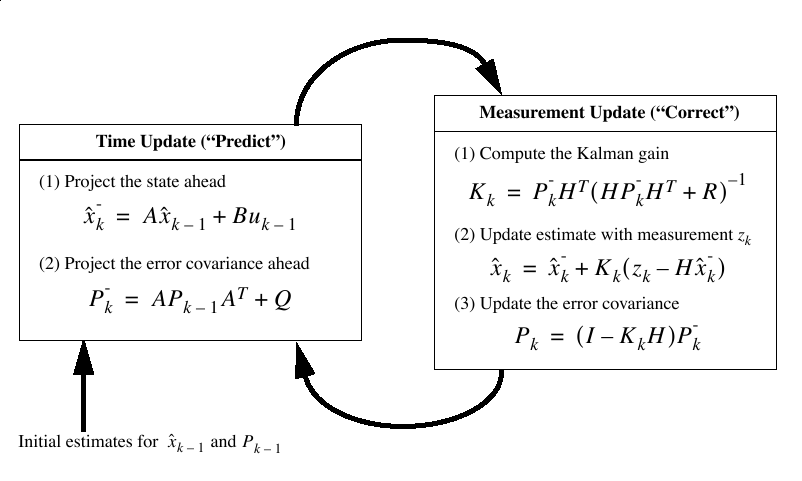
\includegraphics[scale=0.35]{../relazione/figure/cicloKalman.png}
\caption{\tiny \textit{Ciclo di Kalman completo}\label{fig:completeKalman}}
\end{figure}

}

\frame{\frametitle{Il Modello - 1}
Per descrivere il moto dei nostri oggetti ci è sembrata la scelta più semplice rappresentare il
generico moto di un punto nel piano.

\begin{figure}[hb]
\centering
	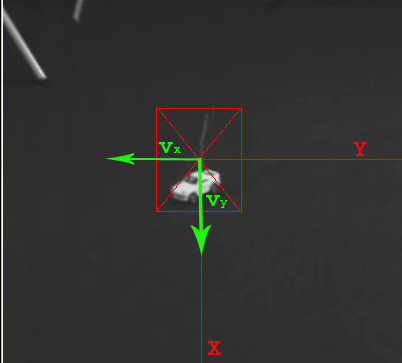
\includegraphics[scale=0.3]{../relazione/figure/motopiano.png}
\caption{\textit{Esempio di vettori di stato moto sul piano}\label{fig:motopiano}}
\end{figure}

\begin{footnotesize}
\begin{itemize}
\item $(x,y)$ è la posizione data secondo le coordinate 
\item $(v_x,v_y)$ è la velocità rispettivamente orizzontale e verticale dell'oggetto nel punto $(x,y)$ 
\end{itemize}
\end{footnotesize}
}


\frame{\frametitle{Il Modello - 2}
\begin{itemize}
\item \begin{math} x= \begin{bmatrix} x \\ y \\ v_{x} \\ v_{y} \end{bmatrix} \end{math}  \footnotesize{è il vettore di stato}\\
\end{itemize}

\begin{itemize}
\item $A = \begin{bmatrix} 1 & 0 & \Delta_{t} & 0 \\ 0 & 1 & 0 & \Delta_{t} \\ 0 & 0 & 1 & 0 \\ 0 & 0 & 0 & 1 \end{bmatrix}$ \footnotesize{è la matrice di transizione del modello}\\
\end{itemize}

\begin{itemize}
\item $B u_{t} = 0$ \footnotesize{sull'oggetto non agiscono forze esterne}
\end{itemize}
}

\frame{\frametitle{Il modello - 3}
\begin{columns}
\column{.50 \textwidth}
\begin{itemize}
\item $Q = \begin{bmatrix} \rho & 0 & 0 & 0 \\ 0 & \rho & 0 & 0 \\ 0 & 0 & \rho & 0 \\ 0 & 0 & 0 & \rho  \end{bmatrix}$ 
\end{itemize}
\column{.50 \textwidth}
\begin{footnotesize}covarianza del processo che rappresenta il rumore sul sistema\end{footnotesize}
\end{columns}

\begin{columns}
\column{.50 \textwidth}
\begin{itemize}
\item $H = \begin{bmatrix} 1 & 0 & 0 & 0 \\ 0 & 1 & 0 & 0 \end{bmatrix}$
\end{itemize}
\column{.50 \textwidth}
\begin{footnotesize}sceglie le componenti dello stato per confrontarlo con la misura\end{footnotesize}
\end{columns}

\begin{itemize}
\item $R = \begin{bmatrix} 0.285 & 0.005 \\ 0.005 & 0.046 \end{bmatrix}$ \begin{footnotesize}definisce il rumore associato alla misura\end{footnotesize}
\end{itemize}
}

\subsection{Condesation}

\frame{\frametitle{Condensation - 1}

E' un'implementazione del Particle Filter, un filtro di tipo Ricorsivo Bayesiano.

\begin{block}{Conditional Density Propagation}
\begin{itemize}
\item E' un algoritmo di tipo probabilistico che risulta molto robusto rispetto a dati rumorosi e a cambiamenti di stato non lineari.
 
\item Permette di essere utilizzato per lo studio di moti descritti anche da modelli complessi di tipo non lineare.

\item Supporta previsoni di tipo multimodale.

\item L'algoritmo utilizza un campionamento casuale e ordinato delle posizioni assunte dall'oggetto nei vari istanti di tempo per modellare funzioni di densità di probabilità arbitrariamente complesse.

\end{itemize}
\end{block}

}

\frame{\frametitle{Condensation - 2}

Utilizza un numero N finito di campioni per approssimare la curva che descrive la distribuzione dei dati $p(x_k \vline z_{1:k})$.\\~\\
Ciascun campione -  sample - consiste di due valori: lo stato e il peso.

\begin{block}{}
Chiamiamo con $H_{t}$ il vettore dei samples all'istante $t$:
\begin{center}
$H_t = \{\overrightarrow{s_1}(t), ... ,\overrightarrow{s_N}(t)\}$
\end{center}

Dove:
\begin{itemize}
\item $\overrightarrow{s_i}(t)= \{\overrightarrow{x_i}(t),p(x_i(t))\}$
\item $\overrightarrow{x_i}(t)$ è la posizione associata al sample $i$ all'istante $t$.
\item $p(\overrightarrow{x_i}(t))$ è la probabilità associata alla posizione $\overrightarrow{x_i}(t)$ che caratterizza il sample $i$
\end{itemize}
\end{block}

}

\frame{\frametitle{Algoritmo - Inizializzazione}
Al primo passo dell'algoritmo si inizializza tutti i samples:
\begin{itemize}
\item Ciascuna posizione può essere scelta in modo casuale secondo una distibuzione uniforme.
\item La probabilità associata a ciascun sample è invece distribuita secondo una gaussiana standard centrata nel valore medio tra il valore massimo e il valore minimo assumibile per la posizione dell'oggetto e la relativa varianza.
\end{itemize}

}


\frame{\frametitle{Algoritmo - passo t}

\begin{itemize}
\item Il sample $\overrightarrow{s_{\bar{i}}}(t)$ con probabilità maggiore è la predizione per il Condensation al passo t.\\
\end{itemize}

Per passare dal vettore $H_{t}$ al vettore $H_{t+1}$ si eseguono questi passi:
\begin{block}{}
\begin{small}
\begin{enumerate}
\item Si campiona la posizione reale dell'oggetto: $\overrightarrow{z}(t)$
\item Si calcola la posizione per ciascun sample secondo lo spostamento dato dal modello dinamico che descrive il moto dell'oggetto: 
\begin{equation}
	\overrightarrow{x_i}(t+1)= f(\overrightarrow{x_i}(t))
\end{equation}
\item Si stima la probabilità $p(\overrightarrow{z}(t))$ secondo la densità di probabilità dei campioni all'istante t centrata in $\overrightarrow{x_{\bar{i}}}(t)$.
\item Per ogni sample è ricalcolata la probabilità condizionata applicando il teorema di Bayes:
\begin{equation}
	p_i(\overrightarrow{x_i}(t+1))= p(\overrightarrow{x_i}(t)\ \mid \overrightarrow{z}(t))
\end{equation}
\end{enumerate}
\end{small}
\end{block}

}


\frame{\frametitle{Il Modello - 4}
La nostra implementazione del Condensation rispetta fedelmete l'algoritmo che è stato prima presentato.\\~\\
Per quanto riguarda il modello dinamico associato si è utilizzata la stessa equazione valida per il tracciamento fatto con il filtro di Kalman:
\begin{block}{}
\begin{small}
\begin{equation}
x_{t+1} = A  x_t
\end{equation}
Dove:
\begin{center}
$A = \begin{bmatrix} 1 & 0 & \Delta_{t} & 0 \\ 0 & 1 & 0 & \Delta_{t} \\ 0 & 0 & 1 & 0 \\ 0 & 0 & 0 & 1 \end{bmatrix} $
\end{center}
\end{small}
\end{block}

}
